\section{Garanties statistiques}


La section précédente été dédiée à l'approche algorithmique du problème: comment, donnés
un ensemble d'entraînement et un espace de décision $\Q$, une fonction de décision
$\hat q:\Q \to \Re$ permettant de prescrire un investissment pouvait être déterminée. Cette
section sera consacrée aux garanties statistiques de cette solution. Dans un premier
temps, une étude de la stabilité de l'algorithme d'optimisation permettra de dériver une
borne de généralisation sur la performance hors-échantillon (Section \ref{b:gen}). Par la
suite, le problème sera approché d'un point probabiliste (en terme de variables
aléatoires) afin de comparer les performances de la décision optimale d'investissement sur
$M$ par rapport à la décision empirique (Section \ref{b:sopt}). Enfin, la Section
\ref{b:dim} portera sur l'influence de la dimensionalité de l'espace $\Q$ sur la qualité
des bornes alors obtenues, et don

Les bornes qui seront dérivées n'auront de signification qu'en terme d'\textit{util},
c'est à dire la dimension de $u(r)$ pour un certain rendement. Comme cette notion n'a en
soi aucune signification tangible, un théorème sera finalement introduit afin d'obtenir
pour chacune des bornes une version sous forme de rendement équivalent.


\paragraph{Hypothèses et discussion}

Certaines hypothèses devront d'abord être formulées afin d'être en mesure d'obtenir des
résultats pertinents: ce sera en fait le prix à payer pour l'absence de contraintes sur la
forme de la distribution $M$, notamment concernant par exemple sa covariance ou la forme
de ses moments d'ordre supérieurs.

\begin{assumption}
  L'amplitude de similarité d'une observation est bornée: pour tout $x \in \X$,
  $\kappa(x,x) \leq \xi^2$.
\end{assumption}
\begin{assumption}
  Le rendement aléatoire est borné: $|R| \leq \rmax$.
\end{assumption}
\begin{assumption}
  \label{hyp:lip}
  Un investisseur est doté d'une fonction d'utilité $u$ concave, monotone et standardisée,
  c'est-à-dire que $u(0) = 0$ et $\partial u(0) \ni 1$\footnote{Ici, $\partial u(r)$ signifie l'ensemble
    des sur-gradients de $u$. Dans le cas dérivable, cela revient à la notion de
    dérivée. Dans le cas simplement continu, $\partial u(r)$ est l'ensemble des fonctions affines
    ``touchant'' à $u(r)$ et supérieures à $u(r)$ pour tout $r$ du domaine). Bien qu'il
    s'agisse d'un ensemble, la situation désigne souvent un sur-gradient optimal par
    rapport aux autres.}. De plus, $u$ est défini sur l'ensemble de $\Re$. Enfin, $u$ est
  $\gamma$-Lipschitz, c'est-à-dire que pour tout $r_1,r_2 \in \Re$,
  $|u(r_1) - u(r_2)| \leq \gamma|r_1-r_2|$.
\end{assumption}

Avant d'aller plus loin, il convient de discuter de la plausiblité de ces
contraintes. Cependant, compte tenu de l'aspect central de la première hypothèse, une
discussion approfondie ne sera abordée qu'à la section \ref{b:dim}.

Pour ce qui est de la seconde hypothèse, si on définit les rendements selon
l'interprétation usuelle d'un changement de prix $p$, \ie, $r = \Delta p/p$, on constatera que
$r$ est nécessairement borné par 0. De plus, selon la période de temps pendant laquelle
$\Delta p$ est mesuré, il y a forcément moyen de limiter l'accroissement dans le prix, pour
autant que $\Delta t$ soit suffisament court.

La troisième hypothèse est davantage contraignante. Elle exclut d'emblée plusieurs
fonctions d'utilité courantes; par exemple l'utilité logarithmique et racine carrée
puisqu'elles ne sont définies que pour $\Re_{+}$. Une utilité quadratique, comme celle de
Markowitz est également inadmissible puisqu'elle est non-monotone. Les utilités de forme
exponentielle inverse $u(r) = \mu(-\exp(-r/\mu)+1)$ quant à elles violent la condition
Lipschitz. On peut cependant définir une utilité exponentielle \textit{à pente contrôlée},
c'est à dire dont la pente devient constante lorsque $r \leq r_0$. Par contre, une utilité
qui serait définie par morceaux linéaires est parfaitement acceptable. Par ailleurs, on
considérera souvent l'utilité \textit{neutre au risque} $\rn: r \mapsto r$ comme un cas
limite à l'ensemble des fonctions d'utilité admissibles.

% \begin{numex}{Fonctions d'utilité Lipschitz}
%   Cette famille de fonctions est paramétrée par $\mu > 0$ et définie par $u(r) = r$ si
%   $r\leq0$ et $u(r)=\mu(1-\exp(-r/\mu))$ dans le cas contraire (\figref{fig:leuu}). On constate
%   les deux cas limites: lorsque $\mu\to\infty$, $u$ se comporte comme une utilité neutre au risque,
%   alors que $\mu\to0$ signifie une attitude d'indifférence aux rendements supérieurs à 0. Par
%   ailleurs, toute fonction exponentielle Lipschitz admet un coefficient Lipschitz unique
%   $\gamma = 1$. Leur simplicité et leur expressivité feront de cette classe d'utilités
%   l'essentiel de l'analyse numérique de ce mémoire.
% \end{numex}

% \begin{figure}
%   \centering
%   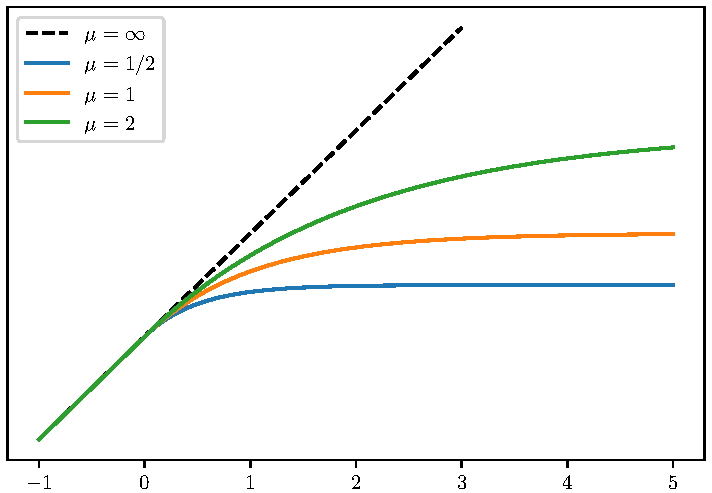
\includegraphics[width=0.7\textwidth]{../../experiments/fig/leuu.pdf}
%   \caption{Fonctions d'utilité Lipschitz}
%   \label{fig:leuu}
% \end{figure}

% \begin{numex}{Copules gaussiennes}
%   Bien que les résultats présentés dans ce travail concernent toute forme de distribution
%   de marché respectant les hypothèses énoncées ci-haut, les simulations numériques qui
%   seront offertes à titre d'exemples seront toutes tirées d'une distribution multivariée
%   liée par une copule gaussienne $\mathcal{C}(\Sigma)$ où $\Sigma \in \Re^{p+1\times p+1}$ est la matrice de
%   corrélation des $p+1$ \textit{marges} de $M$ ($p$ variable d'information $X_j$ et une
%   variable de rendement $R$). Cette flexibilité permet notamment de contraster les
%   résultats lorsque $M$ est strictement bornée ou présente au contraire des queues
%   lourdes, tout en conservant une corrélation identique.
% \end{numex}


\subsection{Bornes de généralisation}
\label{b:gen}


\paragraph{Exposition du problème}

Soit $\Q$ un espace de Hilbert à noyau reproduisant induit par $\kappa$ et soit un ensemble
d'entraînement $\S_n = \{(x_i,r_i)\}_{i=1}^n \sim M^n$ échantilloné à partir de la
distribution de marché. Alors on peut définir \textit{l'algorithme de décision}
$\alg:\M^n \to \Q$ par
\begin{equation}
  \label{b:basic}
  \alg(\S_n) = \argmax_{q \in \Q} \left\{\widehat\EU(\S_n,q) - \lambda\nq{q}^2\right\}.
\end{equation}

Comme on l'a vu, résoudre \eqref{b:basic} est aussi équivalent à
\begin{equation}
  \maximizeEquation[\alpha \in \Re^n]{n^{-1} \sumi u(r_i(\alpha^T\phi)(x_i)) - \lambda \alpha^TK\alpha,}
\end{equation}
où $\phi:\Re^p \to \Re^n$ le vecteur d'application induit par la matrice d'information $\Xi$. La
relation $q = \alpha^T\phi$ permet de passer d'une représentation à l'autre.

La question qui se pose naturellement est de savoir dans quelle mesure une fonction de
décision $\hat q = \alg(\S_n)$ est capable d'offrir à un investisseur une utilité espérée
comparable à celle qu'il aurait observée au sein de l'ensemble d'entraînement. Il serait
aussi souhaitable qu'une telle garantie soit indépendante de l'ensemble d'entraînement
$\S_n$. Autrement dit, on cherche à déterminer une borne probabiliste $\hat\Omega_u$ sur l'erreur de
généralisation de $\hat q = \alg(\S_n)$ valide pour tout $\S_n \sim M^n$:
\begin{equation}
 \hat\zeta_u(\S_n) \leq \hat\Omega_u(n,\ldots),
\end{equation}
où
\begin{equation}
  \label{b:zeta}
  % \hat\zeta(\hat q) = n^{-1}\sumi u(r_i\,\hat q(x_i)) - \E u(R \cdot \hat q(X))
  \hat\zeta_u(\S_n) =  \hEU(\S_n,\alg(\S_n)) - \EU(\alg(\S_n))
\end{equation}
représente l'erreur de généralisation.

Bien que ces résultats soient intéressants d'un point de vue théorique, on veut d'un point
de vue pratique pouvoir garantir au détenteur du portefeuille un intervalle de confiance
sur l'équivalent certain du portefeuille. On cherchera donc une borne $\hat\Omega_e$ telle que
\begin{equation}
  \CE(\S_n,\alg(\S_n)) \geq \hCE(\S_n,\alg(\S_n)) - \hat\Omega_e(n,\ldots).
\end{equation}

% En fait, on peut démontrer que $\hat\Omega_u = \O(n^{-1/2})$, ce qui permet de quantifier la
% ``vitesse'' à laquelle la convergence à lieu.


\paragraph{Intuition et éléments de preuve}

En fait, la motivation derrière ces hypothèses est la suivante: combinées à l'élément de
régularisation, elles parviennent d'une part à borner la perte que peut entraîner la prise
de décision dans le pire cas et d'autre part à borner la différence entre deux fonctions
de décision entraînées sur des ensembles à peu près identiques.

\begin{thm}[Borne sur l'erreur de généralisation (util)]
  L'erreur de généralisation sur $\qh$ est bornée par
  \begin{equation}
  \label{b:borneu1}
  \hEU(\S_n,\alg(\S_n)) - \EU(\alg(\S_n)) \leq \hat \Omega_u,
\end{equation}
où
\begin{equation}
  \label{b:borneu2}
  \hat\Omega_u = \frac{\rmax^2\xi^2}{2\lambda}\left(\frac{\gamma^2}{n} + (2\gamma^2+\gamma+1)\sqrt{\frac{\log(1/\delta)}{2n}}\right).
\end{equation}
\end{thm}

Considérons deux ensembles d'entraînement: $\S_n \sim M^n$ et $\S'_n$, où $\S'_n$ ne diffère
de $\S_n$ que par un seul point (par exemple le $j$-ème point serait rééchantilloné de la
distribution de marché $M$). De l'algorithme $\alg$ on dérivera alors deux décisions:
$\hat q$ et $\hat q'$. Pour $n$ suffisament grand, on peut alors s'attendre à ce que
l'utilité dérivée de ces deux décisions soit relativement proche, et ce, pour toute
observation. On aurait alors une borne $\beta(n)$ telle que pour tout $(x,r) \sim M$,
\begin{equation}
  |u(r\,\hat q(x)) - u(r\,\hat q'(x))| \leq \beta.
\end{equation}
C'est ce qu'on appelle dans la littérature la \textit{stabilité algorithmique}. La plupart
des algorithmes régularisés classiques disposent par ailleurs d'une telle stabilité. En
particulier, le terme de régularisation $\lambda \nq{q}^2$, combiné à la continuité Lipschitz de
$u$ font en sorte que $\beta = \O(n^{-1})$. Par le Lemme \ref{lem:stab}, p.~\pageref{lem:stab}
(une application directe du théorème de Bousquet), on obtient effectivement
\begin{equation}
  \beta \leq \frac{\gamma^2\rmax^2\xi^2}{2\lambda n}.
\end{equation}

Dotée de cette stabilité de $\alg$, la différence dans l'erreur de
généralisation de $\S_n$ et $\S_n'$ peut alors être bornée:
\begin{align}
  |\hat\zeta(\S_n) - \hat\zeta(\S_n')| &= |\EU(\hat q) - \EU(\hat q') + \hEU(\S_n,\hat q) - \hEU(\S_n',\hat q')|\\
                               &\leq |\EU(\hat q) - \EU(\hat q')| + |\hEU(\S_n,\hat q) -
                                 \hEU(\S_n',\hat q')|. \label{b:p1}                         
\end{align}
Or, par le théorème de Jensen appliqué à la fonction valeur absolue, on obtient du premier
terme que
\begin{align}
  |\EU(\hat q) - \EU(\hat q')| &= |\E(u(R \cdot \hat q(X)) - u(R \cdot \hat q'(X)))|\\
                               & \leq \E(|u(R\cdot \hat q(X)) - u(R \cdot \hat q'(X)|)\\
                               & \leq \beta,
\end{align}
par définiton de la stabilité. Quant au deuxième terme de \eqref{b:p1} on peut le borner
de la même façon:
\begin{align}
  &|\hEU(\S_n,\hat q) - \hEU(\S_n',\hat q')|\\
  &\qquad = n^{-1}\left|\sumi \mathbb{I}_{i\neq j}u(r_i\,\hat q(x_i)) + u(r_j\,\hat q(x_j)) - \sumi
    \mathbb{I}_{i\neq j}u(r_i\,\hat q'(x_i)) - u(r_j'\,\hat q'(x_j'))\right|\\
  &\qquad \leq n^{-1}\left(| u(r_j\,\hat q(x_j) - u(r_j'\,\hat q'(x_j'))| +\sumi \mathbb{I}_{i\neq
    j}\big|u(r_i\,\hat q(x_i)) - u(r_i\,\hat q'(x_i))\big|\right)\\
  &\qquad \leq n^{-1}\left(| u(r_j\,\hat q(x_j) - u(r_j'\,\hat q'(x_j'))| + (n-1)\beta\right).
\end{align}
Considérons le premier terme. Par le Lemme \ref{lem:bqhat}, p.~\pageref{lem:bqhat}, on
sait que $\hat q(x) \leq (2\lambda)^{-1}\rmax\xi^2$ et que $|R|\leq\rmax$. On peut donc borner cette
différence par la différence dans l'utilité dérivée par la meilleure décision
d'investissement sur le meilleur rendement et sur le pire rendement. Par hypothèse
Lipschitz et de sur-gradient de 1 à $r=0$, on sait que pour $r>0, u(r)<r$ et que pour
$r<0$, $\gamma r \leq u(r)$. On peut donc conclure que
\begin{align}
  |u(r_j\,\hat q(x_j) - u(r_j'\,\hat q'(x_j')| &\leq u((2\lambda)^{-1}\rmax^2\xi^2) -
                                                 u(-(2\lambda)^{-1}\rmax^2\xi^2)\\
  & \leq (2\lambda)^{-1}(\gamma+1)\rmax^2\xi^2.
\end{align}
Ce qui entraîne donc que
\begin{align}
  |\hEU(\S_n,\hat q) - \hEU(\S_n',\hat q')| &\leq \frac{\gamma+1}{2\lambda n}\rmax^2\xi^2 +
                                              \frac{n-1}{n}\beta\\
                                            &\leq \beta + \frac{\gamma+1}{2\lambda n}\rmax^2\xi^2,
\end{align}
d'où, après quelques simplifications algébriques, on peut enfin tirer que
\begin{equation}
  |\hat\zeta(\S_n) - \hat\zeta(S'_n)| \leq \beta(2\gamma^2 + \gamma + 1).
\end{equation}
Ainsi la différence dans l'erreur de généralisation est de convergence $\O(n^{-1})$. À ce
stade, la démonstration est presque complète, puisqu'en appliquant l'inégalité de
concentration de McDiarmid, on obtient que pour tout $\S_n$,
\begin{equation}
  \pp\{\hat\zeta(\S_n) \geq \epsilon + \E_{\S_n}\hat\zeta(\S_n)\} \leq \exp\left(-\frac{2\epsilon^2}{n\beta^2(2\gamma^2+\gamma+1)^2}\right),
\end{equation}
ce qui revient à dire qu'avec probabilité $1-\delta$:
\begin{equation}
  \hat\zeta(\S_n) < \E_{\S_n}\hat\zeta(\S_n) + \frac{\sqrt{n}\beta(2\gamma^2+\gamma+1)\log(1/\delta)}{2}.
\end{equation}
Or, $\E_{\S_n}\hat\zeta(\S_n) \leq \beta$ (voir \cite{mohri2012foundations} pour une preuve technique
mais complète), d'où on a finalement la borne recherchée.
% \begin{equation}
%   \label{b:borneu1}
%   \hEU(\S_n,\alg(\S_n)) - \EU(\alg(\S_n)) \leq \hat \Omega_u,
% \end{equation}
% où
% \begin{equation}
%   \label{b:borneu2}
%   \hat\Omega_u = \frac{\rmax^2\xi^2}{2\lambda}\left(\frac{\gamma^2}{n} + (2\gamma^2+\gamma+1)\sqrt{\frac{\log(1/\delta)}{2n}}\right).
% \end{equation}


\paragraph{Équivalent certain}

À ce point-ci, il ne reste plus qu'à inverser le domaine de cette garantie pour l'exprimer
en unités de rendements. En effet, si à partir d'un échantillon d'entraînement on a pu
calculer un rendement équivalent $\nhCE = u^{-1}(\nhEU)$, en utilisant le résultat du
Lemme \ref{lem:ce}, p.~\pageref{lem:ce}, un investisseur aura un rendement équivalent hors
échantillon $\nCE$ tel que
\begin{equation}
  \nCE \geq \nhCE - \O(1/(\lambda\sqrt{n})).
\end{equation}
De façon explicite:
\begin{equation}
  \nCE \geq \nhCE - \partial u^{-1}(\nhCE)\cdot \frac{\rmax^2\xi^2}{2\lambda}\left(\frac{\gamma^2}{n} + (2\gamma^2+\gamma+1)\sqrt{\frac{\log(1/\delta)}{2n}}\right).
\end{equation}
Cette borne permet ainsi d'appréhender dans quelle mesure un large échantillonage est
nécessaire pour obtenir un degré de confiance élevé. On notera l'influence de plusieurs
facteurs sur la qualité de la borne (la discussion sur l'influence du terme $\rmax^2\xi^2$
est repoussé à la Section \ref{b:dim}).

Ainsi, la constante $\gamma$ et le terme du sur-gradient inverse $\partial u^{-1}(\nhCE)$ sont tous
deux susceptibles de dégrader considérablement la borne, particulièrement lorsque
l'investisseur est doté d'une utilité très averse au risque; dans des cas extrêmes, par
exemple une utilité exponentielle inverse, ces deux valeurs divergeront très
rapidement. Il convient cependant de prendre note que la constante Lipschitz est
globalement plus importante puisqu'on considère son carré. Il devient alors essentiel de
contrôler l'agressivité de l'algorithme en choisissant des valeurs élevées pour la
régularisation $\lambda$ de manière à chercher une utilité espérée relativement proche de
$u(0)$.

On constate par ailleurs le rôle de premier plan que joue le terme de régularisation. Avec
une régularisation élevée, on obtiendra sans surprise une borne très serrée, mais aux
dépens de la politique d'investissement qui varie selon $\O(1/\lambda)$. Il est donc primordial
de faire une validation croisée sur $\lambda$ pour déterminer le meilleur compromis entre la
variance des résultats et l'objectif à atteindre. La constante de confiance $\delta$ est quant
à elle très performante; une confiance de \num{99.9}\% n'accroît la borne que par un
facteur de \num{2.63}. Enfin, compte tenu du théorème limite centrale, l'ordre de
convergence de $\O(1/\sqrt{n})$ n'a finalement rien de surprenant.\todo{Plus de
  détails...}




\subsection{Bornes de sous optimalité}
\label{b:sopt}


\paragraph{Introduction et hypothèses supplémentaires}

Jusqu'ici, les efforts théoriques ont été déployés pour déterminer comment se comportait
la fonction de décision $\hat q = \alg(\S_n)$ dans un univers probabiliste par rapport à
l'univers statistique dans lequel elle avait été construite. Notre attention va maintenant
se tourner vers la performance de $\hat q$ dans l'univers probabiliste par rapport à la
meilleure décision disponible, c'est à dire la solution $q^\star$ de 
\begin{equation}
  \maximizeEquation[q \in \Q]{\E\,u(R \cdot q(X)).}
\end{equation}

Il convient cependant de réaliser que l'existence d'une borne sur $q^\star$ n'est pas
assurée. En effet, supposons d'une part que l'on dispose d'une utilité neutre au risque
$\rn$, telle que $\rn(r) = r$, et d'autre part que $\E R=0$. Soit $\alpha>0$. On pourrait alors
définir la fonction suivante:
\begin{equation}
  q = \alpha\E(R\,\kappa(X,\cdot))
\end{equation}
On aurait alors, du fait de la linéarité du produit scalaire,
\begin{align}
  \EN(q) &= \E(R\,q(X))\\
         & =\E(R\inp{q,\kappa(X,\cdot)})\\
         & =\E\inp{q,R\,\kappa(X,\cdot)}\\
         & =\inp{q,\E(R\,\kappa(X,\cdot))}\\
         &= \alpha\nq{q}^2 \geq 0.
\end{align}
On peut alors obtenir une utilité espérée non bornée à mesure que $\alpha\to\infty$. Par ailleurs,
ainsi défini, $q$ représente effectivement la covariance entre $R$ et la projection de $X$
dans l'espace dual de $\Q$; par exemple dans le cas d'un noyau linéaire on aurait
$q = \E(RX^T) = \Cov(R,X)$. On sait qu'en espérance l'application de $q$ à $X$ variera de
la même façon que celle de $R$ et donc qu'on aura une utilité infinie, puisque l'utilité
est neutre.

Pour empêcher une telle situation d'exister on introduit l'hypothèse suivante. Elle exclut
toute forme d'utilité à pente constante pour $r \geq r_0$, notamment l'utilité risque neutre.
\begin{assumption}
  L'utilité croît sous-linéairement, ie. $u(r) = o(r)$\footnote{Mathématiquement, on exige
    donc que $u(r)/r \to 0$.}. 
\end{assumption}

Une autre hypothèse est maintenant nécessaire pour s'assurer que $\qs$ soit borné:
l'absence d'arbitrage. D'un point de vue strictement financier, cela fait certainement du
sens en vertu de l'efficience des marchés, version semi-forte\cit. D'un point de vue
théorique, ceci exige en fait qu'il n'y ait pas de région dans $\X$ telle que tous les
rendements s'y produisant soient nécessairement positifs ou négatifs.\todo{Inserer
  image}. Ainsi, même en ayant une conaissance parfaite du monde, il subsistera toujours
un terme de bruit rendant incertains la réalisation des rendements.

\begin{assumption}
  \label{hyp:arb}
  Pour toute région $\mathcal{X}\subseteq\X$,
  \begin{equation}
    \pp\{R \geq 0 \mid X \in \mathcal{X}\} < 1,
  \end{equation}
  et de la même façon avec l'évènement $\pp\{R \leq 0 \mid X \in \mathcal{X}\}$. 
\end{assumption}


\paragraph{Décision optimale finie}

  On veut montrer que $\nq{q^\star}$ est borné. Pour ce faire, on va tout d'abord décomposer
  $q = s\theta$, où on pose $\nq{\theta}=1$ et $s>0$; ainsi on peut poser notre problème
  d'optimisation comme la recherche d'une `direction' $\theta$ et d'une magnitude $s$ dans
  $\Q$. De plus, puisque $\nq{q} = s$, il suffit de montrer que $s^\star$ est borné.

  Notons d'abord que l'hypothèse \ref{hyp:arb} entraîne en particulier qu'il existe
  $\delta > 0$ et $\varrho \geq 0$ tels que
  \begin{equation}
    \pp\{R\cdot \theta(X) \leq -\delta\} > \varrho
  \end{equation}
  pour tout $\theta \in \Q$ tel que $\nq{\theta} = 1$. Définissons maintenant une variable aléatoire à
  deux états: $B = -\delta$ avec probabilité $\varrho$ et $B = \rmax\xi$ avec probabilité
  $1-\varrho$. Puisque $R\cdot \theta(X) \leq \rmax\xi$, on a alors que, pour tout $r \in \R$,
  \begin{equation}
    \pp\{B\geq r\} \geq \pp\{R\cdot \theta(X)\geq r\}
  \end{equation}
  \todo{voir figure a produire.}

  Puisque par hypothèse $u$ est concave et puisque que $B$ domine stochastiquement
  $R\cdot \theta(X)$, on a nécessairement que $\E u(sB) \geq \E u(R\cdot s\theta(X))$, pour tout
  $s > 0$. Or, par hypothèse de sous-linéarité on obtient que
  \begin{align}
    \lim_{s\to\infty}\E u(R\cdot s\theta(X)) &\leq \lim_{s\to\infty}u(sB)\\
                             & = \lim_{s\to\infty}(\varrho u(-s\delta) + (1-\varrho)u(s\rmax\xi))\\
                             & \leq\lim_{s\to\infty}-\varrho s \delta + (1-\varrho)o(s) = -\infty,
  \end{align}
  ce qui démontre bien que $s$ est borné.

\paragraph{Dérivation de la borne}

On cherchera donc à établir une borne $\Omega_u$ sur \textit{l'erreur de sous-optimalité} de
$\hat q \sim \alg(M^n)$:
\begin{equation}
  \EU(\qh) \geq \EU(\qs) - \Omega_u.
\end{equation}

Pour ce faire, on utilisera le résultat suivant, montré par \cit Shalev. En posant
\begin{equation}
  \omega = \frac{4\gamma^2\xi^2(32 + \log(1/\delta))}{\lambda n},
\end{equation}
on obtient qu'avec probabilité $1-\delta$, 
\begin{equation}
\lambda\nq{\qh-\qsl}^2 \leq \EU_\lambda(\qsl)- \EU_\lambda(\qh) \leq \omega.
\end{equation}
De la deuxième inégalité, on obtient alors que
\begin{align}
  \EU(\qh) - \EU(\qsl) & \geq -\omega + \lambda\nq{\qh}^2  -\lambda\nq{\qsl}^2\\
                       & \geq -\omega -2\lambda\nq{\qh}\nq{\qsl-\qh} - \lambda\nq{\qsl-\qh}^2.
\end{align}
Or, pour un même $\delta$, le résultat de Shalev\cit implique que $\nq{\qsl-\qh} \leq
\sqrt{\omega/\lambda}$. De plus, par le lemme \ref{lem:bqhat}, p.~\pageref{lem:bqhat}, $\nq{\qh}\leq
\rmax\xi/(2\lambda)$, d'où on obtient
\begin{equation}
  \EU(\qh) - \EU(\qsl) \geq -2\omega -\rmax\xi\sqrt{\frac{\omega}{\lambda}}.
\end{equation}
Enfin, puisque par définition de $\qsl$, $\EU(\qsl) - \lambda\nq{\qsl}^2 \geq \EU(\qs) -
\lambda\nq{\qs}^2$, on trouve alors que
\begin{equation}
  \EU(\qsl) - \EU(\qs) \geq \lambda\nq{\qsl}^2 - \lambda\nq{\qs}^2 \geq -\lambda\nq{\qs}^2,
\end{equation}
ce qui donne finalement
\begin{align}
  \EU(\qh) &= \EU(\qs) + \EU(\qh) - \EU(\qsl) + \EU(\qsl) - \EU(\qs)\\
           & \geq \EU(\qs) - 2\omega - \rmax\xi\sqrt{\omega/\lambda} - \lambda\nq{\qs}^2.
\end{align}

\paragraph{Équivalent certain et analyse}

À partir du résultat obtenu au dernier paragraphe, on peut à nouveau inverser le domaine
de garantie afin de l'exprimer en rendement équivalent. En définissant $\nCE$ l'équivalent
certain hors échantillon suivant la politique $\qh$ et $\nCE^\star$ l'équivalent certain
optimal compte tenu de l'utilité donnée, l'application directe du Lemme \ref{lem:ce},
permet de garantir une performance de l'ordre de
\begin{equation}
  \nCE \geq \nCE^\star - \O(1/(\lambda\sqrt{n})).
\end{equation}
Plus précisément, avec probabilité $1-\delta$, 
\begin{equation}
  \nCE \geq \nCE^\star - \partial u^{-1}(\nCE) \cdot \left(\lambda\nq{\qs}^2 + \frac{8\gamma^2\xi^2(32+\log(1/\delta))}{n\lambda} + \frac{2\gamma\rmax\xi^2}{\lambda}\sqrt{\frac{32+\log(1/\delta)}{n}}\right)
\end{equation}

Les bornes de sous-optimalité convergent ainsi environ à la même vitesse que celle de
sous-optimalité, c'est-à-dire dans un régime de $\O(1/\sqrt{n})$. Bien sûr, une différence
majeure est la présence de $\nq{\qs}$ qui est a priori impossible à déterminer, dans la
mesure où aucune hypothèse n'est faite sur la distribution de $M$. On constate d'ailleurs
sans surprise qu'une faible valeur de régularisation permet au résultat algorithmique de
se raprocher du résultat optimal, bien que les autres termes de la borne aient un effet
inverse. Par ailleurs, le sur-gradient inverse de $u$ à $\nCE$ ne peut lui non plus être
déterminé précisément, aussi pour estimer la borne on lui substituera $\partial u^{-1}(\nhCE)$. 




\subsection{Garanties et dimensionalité du problème}
\label{b:dim}

Toutes les bornes considérées jusqu'à présent ont été dérivées sans faire apparaître
explicitement la relation qui les lient avec avec la dimension $p$ de l'espace $\Q$;
autrement dit, on a implicitement considéré que $p=o(n)$. Or, si à première vue l'erreur
de généralisation et de sous-optimalité du problème de portefeuille se comportent comme
$\O(1/(\lambda \sqrt{n}))$, dans un contexte ou $p$ est comparable à $n$, on souhaite comprendre
comment l'ajout d'information dans $\Q$ peut venir affecter ces bornes.



\paragraph{Discussion sur la première hypothèse}


Revenons dans un premier temps sur la première hypothèse qu'on a employé allègrement dans
nos résultats; celle-ci stipule que $\kappa(x,x) \leq \xi^2$. Pour les espaces de décision affines,
par exemple ceux engendrés par les noyaux de la forme $\kappa(x_1,x_2) = f(\|x_1-x_2\|)$, cette
propriété est naturellement observée puisqu'alors $\kappa(x,x) = f(0)$, peu importe la taille
de $\X$. Pour d'autres types de noyaux, par exemple les décisions linéaires
$\kappa(x_1,x_2) = x_1^Tx_2$, il devient alors nécessaire de borner le support de $X$ pour
respecter la condition. Deux approches peuvent alors être employées : soit chaque variable
d'information est bornée individuellement, soit on borne simplement $\kappa(X,X)$ par une borne
probabiliste.

Le premier cas se prête bien à la situation où on dispose d'une bonne compréhension des
variables d'information et de leur distribution. Par exemple, $X_j$ peut naturellement
et/ou raisonnablement reposer sur un support fini; pour d'autres types de distributions,
par exemple les variables normales et sous-normales (dominées stochastiquement par une
variable normale), on peut borner avec un haut degré de confiance la déviation de leur
espérance. Les cas problématiques seront plutôt présentés par des variables $X_j$
présentants des moments supérieurs élevés. En pratique, on pourra alors soit
\textit{saturer} l'information par une borne arbitraire, \ie\ en posant
$\tilde X_j = X_j(\nu_j/|X_j|)$, puis en ajoutant une nouvelle dimension d'information
vrai/faux indiquant si la borne a été atteinte, ou simplement décider de l'incorporer
telle qu'elle, mais en n'ayant alors aucune garantie sur les performances hors
échantillon. Pour un noyau linéaire, si chaque variable $|X_j| \leq \nu_j$, alors par le
théorème de Pythagore on a simplement que $\|X\|^2 \leq \|\nu\|^2 = \xi^2$. On remarquera alors
que $\xi^2 = \O(p)$. Pour les noyaux polynomiaux d'ordre $k$, ce serait plutôt
$\xi^2 = \O(p^k)$.

Penchons-nous un moment sur le cas linéaire. La situation où $X$ dispose d'une borne
explicite sur son support peut en fait être relaxée, moyennant que chacune des composantes
soient indépendantes l'une à l'autre et que leur carré soient de forme
sous-exponentielle\footnote{Voir Boucheron et/ou Wainwright et/ou définir
  brièvement}. Sous sa forme généralisée, l'inégalité de Bernstein implique qu'avec haute
probabilité,
\begin{equation}
  \pp\{|\|X\|^2 - \E\|X\|^2| \geq t\} \leq \exp\left(\frac{t^2}{\O(p)}\right).
\end{equation}
Autrement dit, à mesure que $p$ est grand, la norme $\|X\|^2$ sera concentrée autour de
son espérance. Si $\E X_j=0$, alors $\|X\|^2 \approx \E\|X\|^2 = \sumj \Var X_j = \O(p)$, et on
aura donc une borne $\xi^2 = \O(p)$, mais nettement plus forte que celle considérée au
dernier paragraphe, puisque les bornes deviennent alors inutiles. De plus, l'ajout d'une
seule dimension d'information vient automatiquement rendre inexacte la borne statique
$\xi^2$. 

Dans un contexte où $p$ est de l'ordre de $n$, les bornes dérivées aux deux dernières
sous-sections peuvent donc se révéler trompeuses, puisqu'elles suggèrent à un potentiel
investisseur des garanties ne dépendant que de $n$. En particulier, puisque toutes nos
bornes sont en fait de la forme $\Omega = \O(\xi^2/\lambda\sqrt{n})$, il serait plus exact de postuler
l'existence d'une variable $\xi^2$ telle que les bornes se comportent en fait selon la
dynamique
\begin{equation}
  \Omega = \O(p/\lambda\sqrt{n}).
\end{equation}
En particulier, dans des régimes où $\sqrt{n}=\O(p)$, il devient impossible d'avoir des
bornes convergeant vers 0, celles-ci restant en fait stationnaires. En outre, si
$\sqrt{n}=o(p)$, par exemple si $p=\O(n)$, alors une divergence devient assurée.

Cependant, cette discussion n'est valide que dans le cas particulier des noyaux
linéaires. Les noyaux gaussiens conservent quant à eux une indépendance par rapport à la
dimensionalité, alors que les noyaux polynomiaux l'exacerbent; pour un noyau de degré $k$
il devient plus juste d'indiquer
\begin{equation}
  \Omega = \O(p^k/\lambda\sqrt{n}).
\end{equation}


\paragraph{Introduction au cas linéaire}

\todo{Ne pas lire cette section!!}
Pour le moment, nous allons considérer le cas plus simple où $\Q = \X^*$, c'est à dire que
le problème revient simplement à 
\begin{equation}
  \maximizeEquation[q \in \Re^p]{n^{-1}\sumi r_i\,q^Tx_i - \lambda\|q\|^2.}
\end{equation}
Pour simplifier la présentation, une utilité neutre au risque sera considérée comme cas
limite au problème plus général (voir lemme de borne\cit).

D'un point de vue probabiliste, on peut définir $\qsh$ comme la solution de
\begin{equation}
  \maximizeEquation[q \in \Re^p]{\E(R\,X^Tq) - \lambda\|q\|^2,}
\end{equation}
d'où on tire
\begin{equation}
  q^\star_\lambda = \frac{1}{2\lambda}\Cov(R,X),
\end{equation}
puisque les deux variables sont centrées. On retrouve alors l'inégalité montrée en lemme
\cit (nécessaire??)
Considérons maintenant $P$ le rendement aléatoire obtenu en utilisant la décision $\qsh$:
\begin{equation}
  P = \frac{1}{2\lambda}R\,X^T\Cov(R,X).
\end{equation}
On a alors $\E P = 1/2\lambda\,\Cov^2(R,X)$.

Puisque toutes nos variables sont centrées et réduites,
\begin{equation}
  \Cov(R,X) = \sumj\E R\,X_j.
\end{equation}

En supposant que notre problème est pleinement déterminé en supposant l'existance d'une
matrice $A$ telle que $R = AX$


\subsection{Note bibliographique}

La théorie de la stabilité algorithmique remonte en fait aux années 70 avec les travaux de
Luc Devroye appliqués à l'algorithme des $k$ plus proches voisins\cit. Jusqu'alors, les
bornes de généralisation étaient présentées pour toute décision $q \in \Q$ (ie
Vapnik). Bousquet\cit a été le premier a présenter des résultats dans des espaces de
Hilbert à noyau reproduisant. La démonstration est fortement inspirée de l'excellente
référence \cite{mohri2012foundations}. La démonstration de la borne sur la décision bornée
est un résultat inédit, dûe à Delage dans le cas linéaire. On doit également à Rudin
l'idée de la dimensionalité sur la qualité des garanties, et plus généralement l'idée
d'employer une fonction de perte pour parvenir à autre chose qu'une question de
régression/classification comme c'est souvent le cas.



\subsection{Lemmes}

\todo{Ordonner les lemmes selon l'ordre dans lequel ils sont invoqués.}

\begin{lemme}[Stabilité]
\label{lem:stab}
On montre ici que
\begin{equation}
  \beta \leq \frac{(\gamma\rmax\xi)^2}{2\lambda n}.
\end{equation}
\end{lemme}


\begin{lemme}[Décision neutre au risque comme cas limite]
  \label{lem:rn}
  Soient $\qu$ la solution de
  \begin{equation}
    \maximizeEquation[q \in \Q]{\hEU_\lambda(q)}
  \end{equation}
  et $\qn$ la solution de
  \begin{equation}
    \maximizeEquation[q \in \Q]{\hEN_\lambda(q),}
  \end{equation}
  où $\hEN(q):=n^{-1}\sumi r_i\,q(x_i)$. On note tout d'abord avec l'inégalité de Jensen
  que $u(\hEN(\qu)) \geq \hEU(\qu) \geq \lambda\nq{\qu}^2 \geq 0$. Mais puisque $u$ a un sur-gradient de
  1 à $0$, on déduit que $u(x) \geq 0$ entraîne $x \geq u(x)$. On a ainsi
  $\hEN(\qu) - \lambda\nq{\qu}^2 \geq 0$. Mais comme $\qn$ maximise $\hEN_\lambda$, on obtient
  \begin{equation}
    \hEN(\qn) - \lambda\nq{\qn}^2 \geq \hEN(\qu) - \lambda\nq{\qu}^2 \geq 0,
  \end{equation}
  d'où on tire finalement $\nq{\qu} \leq \nq{\qn}$.
\end{lemme}


\begin{lemme}[Borne sur la décision algorithmique]
  \label{lem:bqhat}
  On va ici démontrer que la décision $\hat q(x)$ est bornée, et ce, pour tout $x \in \X$ et
  pour toute solution $\hat q$ de
  \begin{equation}
    \label{b:l1}
    \maximizeEquation[q \in \Q]{\hEU_\lambda(q).}
  \end{equation}
  Pour ce faire, on va mettre à profit la propriété reproductive de $\Q$ induite par
  $\kappa$ qui stipule que
  \begin{equation}
    q(x) = \langle q, \kappa(x,\cdot)\rangle_{\Q} \leq\nq{q}\,\sqrt{\kappa(x,x)},
  \end{equation}
  où l'inégalité découle de l'inégalité Cauchy-Schwartz appliquée au produit interne de
  $\Q$.  On rappelle que, par hypothèse, $\forall x\in\X, \kappa(x,x) \leq \xi^2$; il suffit donc de borner
  $\nq{q}$. De plus, par le Lemme \ref{lem:rn}, il suffit en fait de borner la solution de
  $\hEN_\lambda(q)$. Mais,
  \begin{align}
    \hEN_\lambda(q) &= n^{-1}\sumi r_i\,q(x_i) - \lambda\nq{q}^2\\
              & \leq n^{-1}\sumi r_i\sqrt{\kappa(x_i,x_i)}\nq{q} - \lambda\nq{q}^2\\
              & \leq \rmax \xi \nq{q} - \lambda\nq{q}^2.
  \end{align}
  Puisque l'expression $\rmax \xi \nq{q} - \lambda\nq{q}^2$ est quadratique, elle atteint son
  maximum à
  \begin{equation}
    \nq{q} = \frac{\rmax \xi}{2\lambda},
  \end{equation}
  on en conclut que $\nq{\hat q} \leq (2\lambda)^{-1}\rmax\xi$ et donc que
  \begin{equation}
    \hat q(x) \leq \frac{\rmax\xi^2}{2\lambda}.
  \end{equation}
\end{lemme}



\begin{lemme}[Forte concavité]
  L'objectif est fortement concave, que ce soit sous sa version statistique $\hEU_\lambda$ ou
  probabiliste $\EU_\lambda$. Autrement dit, pour tout $\alpha \in [0,1]$, on a
  \begin{equation}
    \EU_\lambda(tq_1 + (1-\alpha )q_2) \geq \alpha \EU_\lambda(q_1) + (1-\alpha)\EU_\lambda(q_2) + \lambda \alpha(1-\alpha)\nq{q_1-q_2}^2,
  \end{equation}
  et de même pour $\hEU_\lambda$. Effectivement, puisque $u$ est concave et $\nq{\cdot}^2$ est
  convexe, on a successivement:
  \begin{align}
    & \EU_\lambda(\alpha q_1 + (1-\alpha )q_2)\\
    &\qquad= \E u(R\cdot (\alpha q_1+(1-\alpha )q_2)(X)) - \lambda\nq{\alpha q_1 + (1-\alpha)q_2}^2\\
    &\qquad= \E u(\alpha (R\cdot q_1(X)) + (1-\alpha )(R\cdot q_2(X)))- \lambda\nq{\alpha q_1 + (1-\alpha)q_2}^2\\
    &\qquad\geq \E(\alpha  u(R\cdot q_1(X)) + (1-\alpha )u(R\cdot q_2(X))) - \lambda\nq{\alpha q_1 + (1-\alpha)q_2}^2\\
    &\qquad= \alpha\EU(q_1) + (1-\alpha)\EU(q_2) - \lambda\nq{\alpha q_1 + (1-\alpha)q_2}^2\\
    &\qquad= \alpha\EU_\lambda(q_1) + (1-\alpha)\EU_\lambda(q_2) - \lambda(\nq{\alpha q_1+(1-\alpha)q_2}^2 - \alpha\nq{q_1}^2 -
      (1-\alpha)\nq{q_2}^2).
  \end{align}
  Mais d'autre part,
  \begin{align}
    &-\lambda\nq{\alpha q_1 + (1-\alpha)q_2}^2 + \lambda\alpha\nq{q_1}^2+\lambda(1-\alpha)\nq{q}^2\\
    &\qquad = \lambda\alpha(1-\alpha)(\nq{q_1}^2 + \nq{q_2}^2 - 2\langle q_1,q_2\rangle)\\
    &\qquad = \lambda\alpha(1-\alpha)\nq{q_1-q_2}^2,
  \end{align}
  Ce qui complète la démonstration. La dérivation demeure exactement la même lorsqu'on
  considère $\hEU_\lambda$.
\end{lemme}


\begin{lemme}[Borne sur l'équivalent certain]
  \label{lem:ce}
  Soient $\nCE_1 = u^{-1}(\nEU_1)$ et $\nCE_2 = u^{-1}(\nEU_2)$ et soit une borne $\Omega_u$ telle
  que
  \begin{equation}
    \nEU_1 \geq \nEU_2 - \Omega_u.
  \end{equation}
  Par définition du sur-gradient, pour tout $r \in \Re$,
  $u(r+\Delta) \leq u(r) + \Delta\cdot\partial u(r)$. Donc en posant
  $\Delta = \nCE_1 - \nCE_2$ et $r=\nCE_2$, on obtient ces deux inégalités:
  \begin{equation}
    -\Omega_u \leq \nEU_1 - \nEU_2 = u(\nCE_1) - u(\nCE_2) \leq \partial u(\nCE_2)(\nCE_1 - \nCE_2).
  \end{equation}
  On trouve ainsi:
  \begin{equation}
    \nCE_1 \geq \nCE_2 - \Omega_u\cdot \partial u^{-1}(\nCE_2).
  \end{equation}
  Typiquement, $\nCE_1$ et $\nEU_1$ seront des quantités inobservables, alors que $\nCE_2$
  et $\nEU_2$ seront des quantités calculables. De plus, si $\partial u^{-1}(\nCE_2)$ comporte
  plusieurs éléments (\eg\ si la dérivée de $u$ est discontinue à $\nCE_2$), on choisira
  l'élément le plus favorable; la plupart du temps ce sera équivalent à
  $\lim_{r\to\nCE_2^{-}}1/u'(r)$ dans la région où $1/u'(r)$ est défini. Enfin, on note que
  cette limite existe puisque $u$ est strictement monotone, et donc sa pente ne s'annule
  nulle part.
\end{lemme}


\begin{lemme}[Généralisation du lemme de Hoeffding]
  \label{b:lem:hoeffding}
  Ce lemme généralise le lemme de Hoeffding à un espace vectoriel de dimension arbitraire
  $\Q$. Soit un vecteur aléatoire $Q\in\Q$ tel que $\nq{Q}\leq\beta$ et $\E Q = 0$. Alors pour tout
  $t\in\Q$, 
  \begin{equation}
    \E e^{\inp{t,Q}} \leq \exp\left(\frac{\beta^2\|t\|^2}{2}\right).
  \end{equation}
  En effet, on sait que par définition de la convexité de la fonction exponentielle, pour
  tout $s\in[0,1]$,
  \begin{equation}
    \exp(sa + (1-s)b) \leq s\exp a + (1-s)\exp b.
  \end{equation}
  Donc en définissant $g:\{q \in \Q:\|q\|\leq\beta\}\to[0,1]$ par
  \begin{equation}
    g(q) = \frac{1}{2}\left(\frac{\inp{t,q}}{\beta\|t\|} + 1\right)
  \end{equation}
  et en posant $a = \beta\|t\|$ et $b = -\beta\|t\|$, alors pour tout $q \in \Q$,
  \begin{gather}
    a g(q) = \frac{1}{2}(\inp{t,q} + \beta\|t\|),\\
    b (1-g(q)) = - \frac{1}{2}(\beta\|t\| - \inp{t,q}),
  \end{gather}
  et donc
  \begin{equation}
    \exp(ag(q) + (1-g(q))b) = e^{\inp{t,q}}.
  \end{equation}
  La branche droite de l'inégalité devient quant à elle
  \begin{equation}
    \left(\frac{\inp{t,q}}{\beta\|t\|} + 1\right)e^{\beta\|t\|} + \left(1-\frac{\inp{t,q}}{\beta\|t\|}\right)e^{-\beta\|t\|}
  \end{equation}
  et donc, puisque $\E\inp{t,Q} = \inp{t,\E Q} = 0$, 
  \begin{align}
    \E e^{\inp{t,Q}} &\leq \E\left(\left(\frac{\inp{t,Q}}{\beta\|t\|} + 1\right)e^{\beta\|t\|} +
                       \left(1-\frac{\inp{t,Q}}{\beta\|t\|}\right)e^{-\beta\|t\|}\right)\\
                     &= e^{\beta\|t\|} + e^{-\beta\|t\|}\\
                     &= e^{\phi(\beta\|t\|)}
  \end{align}
  où $\phi(x) = \log(e^{x} + e^{-x})$. Or, avec le résultat de \cite{mohri2012foundations},
  p.~370, on a $\phi(x) \leq x^2/2$, d'où on tire le résultat annoncé.
\end{lemme}

\begin{lemme}[Généralisation de la borne de Chernoff]
  \label{b:lem:chernoff}
  Ce lemme généralise la borne de Chernoff à un espace vectoriel de dimension arbitraire
  $\Q$. Soit un vecteur aléatoire $Q \in \Q$. Alors l'évènement $\|Q\| \geq \epsilon$ aura lieu si et
  seulement s'il existe $t \in \Q$, $\|t\|=1$ tel que $\inp{t,Q} \geq \epsilon$. Ainsi, pour tout
  $s>0$, en employant l'inégalité de Markov, 
  \begin{align}
    \pp\{\|Q\| \geq \epsilon\} &= \pp\{s\inp{t,Q} \geq s\epsilon\} = \pp\{e^{s\inp{t,X}} \geq e^{s\epsilon}\}\\
                     &\leq e^{-s\epsilon}\E e^{\inp{t,Q}}.
  \end{align}
\end{lemme}

\begin{lemme}[Généralisation de l'inégalité de McDiarmid]
  \label{b:lem:mcdiarmid}
  L'inégalité de McDiarmid peut également se généraliser à des fonctions prenant leurs
  valeurs dans des espaces vectoriels À élaborer!

  Soit une distribution $\mathscr{F}$ à valeur dans un espace quelconque $\bm F$, un
  espace vectoriel $\Q$ et une fonction $f:\bm F^n\to \Q$. S'il existe une constante
  $c\in\Re$ telle que pour deux ensembles d'échantillons \iid\ $\S_n \sim \mathscr{F}^n$ et
  $\S'_n$, où $\S_n$ et $\S'_n$ ne diffèrent que d'un seul point rééchantilloné de
  $\mathscr{F}$, on a
  \begin{equation}
    \|f(\S_n) - f(\S'_n)\| \leq c,
  \end{equation}
  alors pour tout échantillon aléatoire $\S_n\sim\mathscr{F}^n$, 
  \begin{equation}
    \pp\{\|f(\S_n) - \E f(\S_n)\| \geq \epsilon\} \leq \exp\left(-\frac{2\epsilon^2}{nc^2}\right).
  \end{equation}
\end{lemme}


\begin{lemme}[Borne sur la décision]
  \label{b:lem:qhnorm}
  Considérons le cas d'une utilité neutre au risque puisqu'on sait que toute solution à
  $\max_q\EU_\lambda(q)$ sera bornée par celle de $\max_q\EN_\lambda(q)$.  La stabilité de
  l'algorithme $\alg$ fournie par \cite{bousquet2002stability} établit que pour deux
  échantillons $\S_n$ et $\S_n'$ tirés de $M^n$ et ne différant que d'un seul point,
  \begin{equation}
    \|\alg(\S_n) - \alg(\S'_n)\| \leq \frac{\rmax\xi}{\lambda n}.
  \end{equation}
  En posant $\qh \sim \alg(M^n)$, on peut donc appliquer directement le résultat de
  l'inégalité de McDiarmid (\lemref{b:lem:mcdiarmid}) pour obtenir avec probabilité
  $1-\delta$ que
  \begin{equation}
    \|\qh - \E\alg(\S_n)\| \leq \frac{\rmax\xi}{\lambda}\sqrt{\frac{\log(1/\delta)}{2n}}.
  \end{equation}
  Or, $\alg$ est un estimateur non-biaisé de $\qsl$. En effet, pour une utilité neutre au
  risque,
  \begin{align}
    \E\alg(\S_n) &= \E_{M^n}\left(\frac{1}{2n\lambda}\sumi r_i\,\kappa(\cdot,x_i)\right)\\
                 & =\frac{1}{n}\sumi \frac{1}{2\lambda}\E_M(R\,\kappa(\cdot,X))\\
                 & =\frac{1}{n}\sumi \qsl\\
                 &=\qsl.
  \end{align}
  On obtient ainsi
  \begin{equation}
    \|\qh - \qsl\| \leq \frac{\rmax\xi}{\lambda}\sqrt{\frac{\log(1/\delta)}{2n}}.
  \end{equation}
\end{lemme}

\begin{numex}{Convergence de $\qh$ vers $\qsl$}
  La propriété du \lemref{b:lem:qhnorm} s'illustre particulièrement bien dans le cas où
  $M$ n'est formé à ses marges que de distributions Rademacher. Ainsi, dans la
  \figref{fig:normqhqsl}, une distribution de marché à deux variables d'information
  indépendantes et toutes deux de corrélation $\rho=0.5$ avec $R$ sous copule gaussienne a
  été simulée \num{10000} fois, pour constituer une ``vraie'' distribution pour laquelle
  $\qsl$ peut être calculé; \num{2000} échantillons de $\S_n$ ont été simulés.
\begin{figure}
  \centering
  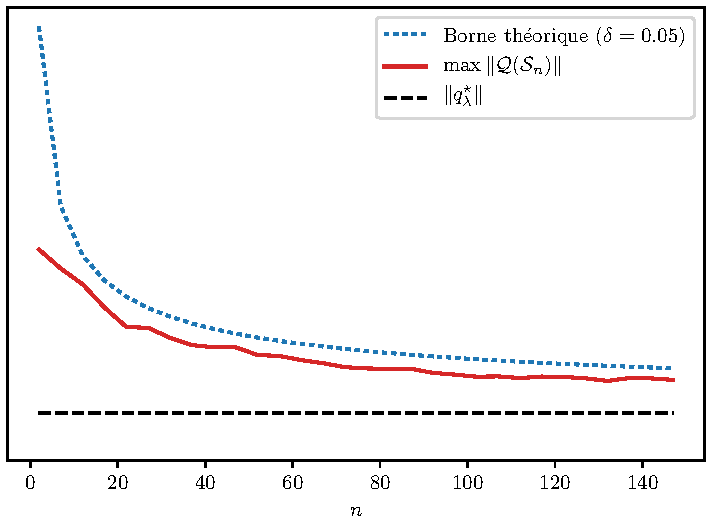
\includegraphics[width=0.7\textwidth]{../../experiments/fig/normqhqsl.pdf}
  \caption{Illustration du \lemref{b:lem:qhnorm}.}
  \label{fig:normqhqsl}
\end{figure}
\end{numex}


\begin{lemme}
  La solution $\qh_1$ de
  \begin{equation}
    \maximizeEquation[q \in \Q]{\EN_\lambda(q) = \hE\braket{q|t} - \tfrac{\lambda}{2}\|q\|^2.}
  \end{equation}
  est donnée par
  \begin{equation}
    \bra{\qh_1} = \lambda^{-1}\hE\bra{t}
  \end{equation}
  où $\bra{x_i} = \kappa(x_i,\cdot)$ est l'élément dual de $x$ sous $\Q$. Sous un noyau linéaire cela
  revient donc à 
  \begin{equation}
    \qh_1^T = \lambda^{-1}\hat\E(r^Tx)
  \end{equation}
  c'est à dire la covariance décentrée entre $r$ et $x$. On observera aussi que
  \begin{equation}
    \EN = \lambda\braket{\qh_1|\cdot}.
  \end{equation}
  et donc que
  \begin{equation}
    \EN(\qh_1) = \lambda\|\qh_1\|^2.
  \end{equation}
\end{lemme}

\begin{proof}
  Si on considère un déplacement de décision $\qh_1 + \Delta q$, alors par linéarité le premier
  terme de l'objectif devient $\EN(\qh_1+\Delta q) = \EN(\qh_1) + \EN(\Delta q)$ et le terme de
  régularisation devient 
  \begin{equation}
    -\lambda/2\|\qh_1 + \Delta q\|^2 = -\lambda/2\|\qh_1\|^2 - \lambda\braket{\qh_1|\Delta q} - \lambda/2\|\Delta q\|^2.
  \end{equation}
  On a donc
  \begin{align}
    \EN_\lambda(\qh_1)  - \EN_\lambda(\qh_1+\Delta q) &= -\EN(\Delta q) + \lambda\braket{\qh_1|\Delta q} + \lambda/2\|\Delta q\|^2\\
                                     &= -\lambda\braket{\qh_1|\Delta q} + \lambda\braket{\qh_1|\Delta q} +
                                       \lambda/2\|\Delta q\|^2\\
                                     &= \lambda/2\|\Delta q\|^2 \geq 0,
  \end{align}
  Ce qui entraîne $\EN_\lambda(\qh_1) \geq \EN_\lambda(\qh_1 + \Delta q)$.
\end{proof}

\begin{lemme}[Borne sur la décision utilitaire]
  \label{lem:rn}
  Pour toute fonction d'utilité $u$ respectant les hypothèses,
  \begin{equation}
    \|\qh_1\| \geq \|\qh_u\|.
  \end{equation}
  Ce lemme entraîne notamment que l'utilité en échantillon $\hEU(\qh_u) \leq \hEN(\qh_1)$:
  puisque $u(x) \leq x$,
  \begin{align}
    \hEU(\qh_u)&\leq \hEN(\qh_u) = \lambda\braket{\qh_1,\qh_u} \leq \lambda\|\qh_1\|\|\qh_u\| \leq \lambda\|\qh_1\|^2\\
               &=  \hEN(\qh_1)
  \end{align}
\end{lemme}

\begin{proof}
  On note tout d'abord avec l'inégalité de Jensen que
  $u(\hEN(\qu)) \geq \hEU(\qu) \geq \lambda/2\|\qu\|^2 \geq 0$ puisque la valeur de l'objectif
  $\hEN_\lambda(q)$ est d'au moins 0 à $q=0$. Mais puisque $u$ a un sur-gradient de 1 à
  $0$, on déduit que $u(x) \geq 0$ entraîne $x \geq u(x)$. On a ainsi
  $\hEN(\qu) - \lambda/2\nq{\qu}^2 \geq 0$. Ce qui entraîne alors que
  \begin{equation}
    \lambda\braket{\qh_1|\qh_u} \geq \lambda/2\|\qh_u\|^2
  \end{equation}
  Mais par Cauchy-Schwartz, on a aussi
  \begin{equation}
    \|\qh_1\|\|\qh_u\| \geq \braket{\qh_1,\qh_u} \geq \|\qh_u\|^2/2
  \end{equation}
  Et donc
  \begin{equation}
    \|\qh_1\| \geq \|\qh_u\|/2.\qedhere
  \end{equation}
\end{proof}


\begin{lemme}
L'erreur de généralisation du problème averse au risque est bornée par celle du problème
neutre au risque:
\begin{equation}
  \hEU(\qu) - \EU(\qu) \leq \gamma(\hEN(\qn) - \EN(\qn)).
\end{equation}
\end{lemme}
\begin{proof}
  Puisque $u$ est monotone, on peut tout d'abord noter que pour tout $r+\Delta \in \R$, on a
  l'inégalité $u(r+\Delta) \leq u(r) + \Delta \partial u(r)$. Ainsi, pour deux variables aléatoires $R_1,R_2 \in
  \R$, en posant $\Delta = R_1-R_2$, on a nécessairement
  \begin{equation}
    u(R_1) - u(R_2) \leq \partial u(R_2) (R_1 -R_2) \leq \gamma(R_1 - R_2),
  \end{equation}
  par définition du coefficient Lipschitz. On tire donc
  \begin{equation}
    \E u(R_1) - \E u(R_2) \leq \gamma(\E R_1 - \E R_2). 
  \end{equation}
  En appliquant cette inégalité aux opérateurs $\hEU$ et $\EU$ on obtient alors
  \begin{align}
    \hEU(\qu) - \EU(\qu) &\leq \gamma(\hEN(\qu) - \EN(\qu))\\
                         &= \gamma\lambda(\braket{\qh_1|\qu} - \braket{\qsl|\qu}).
  \end{align}
  Mais par le \lemref{lem:rn}, $\braket{\qh_1|\qu} \geq 0$ et $\|\qu\| \leq 2\|\qh_1\|$. 
\end{proof}







%%% Local Variables:
%%% mode: latex
%%% TeX-master: "../memoire/memoire.tex"
%%% End:
